%%!TEX root = ./UserManual.tex
\chapter{Simulator}
\label{chap:simulator}


%%%%%%%%%%%%%%%%%%%%%%%%%%%%%%%%%%%%%%%%%%%%%%%%%%%%%%%%%%%%%%%%
% Workspace
%%%%%%%%%%%%%%%%%%%%%%%%%%%%%%%%%%%%%%%%%%%%%%%%%%%%%%%%%%%%%%%%
\section{Workspace}

By default, stride is installed in \texttt{./target/installed/} inside de project directory though this can be modified using the CMakeLocalConfig.txt file (example is given in \texttt{./src/main/resources/make}). Compilation and installation of the software will create the following files and directories: (illustrated in Figure \ref{fig:workspace}):

\begin{compactitem}
    \item Binaries 
    		in directory \texttt{./target/installed/bin}
      	\begin{itemize}
        		\item $stride$: executable.
			\item $gtester$: regression tests for the sequential code.
        		\item $sim\_wrapper.py$: Python simulation wrapper  		
        \end{itemize}
    \item Configuration files (json)
      	in directory \texttt{./target/installed/config}
      	\begin{itemize}
        		\item $config\_ar\_alaska.json$: configuration file for the sim\_wrapper to perform Alaska simulations with different attack rates.
			\item $config\_ar\_brooklyn.json$: configuration file for the sim\_wrapper to perform Brooklyn simulations with different attack rates.
        		\item $config\_ar\_nassau.json$: configuration file for the sim\_wrapper to perform Nassau simulations with different attack rates.
        \end{itemize}
    \item Input data files (csv)
      	in directory \texttt{./target/installed/data}
      	\begin{itemize}
        		\item $alaska\_synt\_pop\_sorted$: Synthetic population data extracted from the 2005-2009 U.S. Synthetic Population Database (Version 1) from RTI International for Alaska. The person data is sorted according to day cluster (first) and household (second).
		 	\item $brooklyn\_synt\_pop\_sorted$: Synthetic population data extracted from the 2010 U.S. Synthetic Population Database (Version 1) from RTI International for Brooklyn, New York \cite{wheaton2014a,wheaton2014b}. The person data is sorted according to day cluster (first) and household (second).
       		\item $nassau\_synt\_pop\_sorted$: Synthetic population data extracted from the 2010 U.S. Synthetic Population Database (Version 1) from RTI International for Nassau, New York \cite{wheaton2014a,wheaton2014b}. The person data is sorted according to day cluster (first) and household (second).
        \end{itemize}
    \item Documentation files
      	in directory \texttt{./target/installed/doc}
      	\begin{itemize}
        		\item Reference manual
        		\item User manual
        \end{itemize}
\end{compactitem}


\begin{figure}[h]
	\begin{center}
		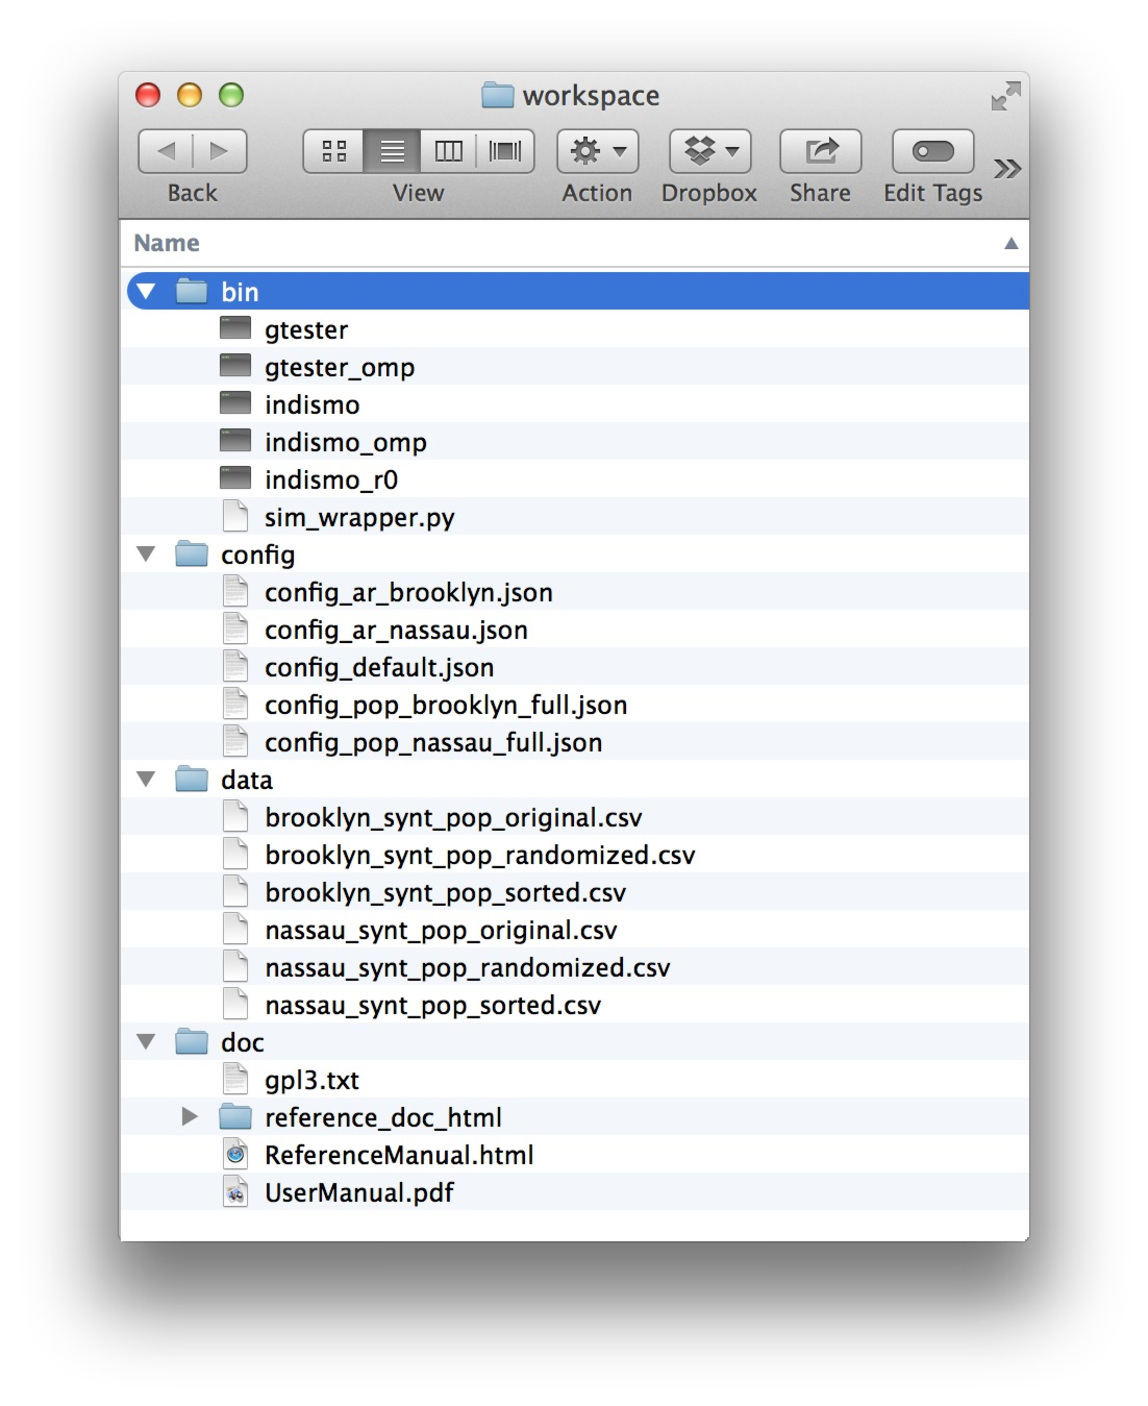
\includegraphics[width=0.55\textwidth]{images/screen_shot_workspace_dir.pdf}  
	\end{center}
	\caption{Screen shot of the workspace directory.}
	\label{fig:workspace}
\end{figure}



%%%%%%%%%%%%%%%%%%%%%%%%%%%%%%%%%%%%%%%%%%%%%%%%%%%%%%%%%%%%%%%%
% Run
%%%%%%%%%%%%%%%%%%%%%%%%%%%%%%%%%%%%%%%%%%%%%%%%%%%%%%%%%%%%%%%%
\section{Run the simulator}


From the workspace directory, the simulator can be started with default configuration using the command \mbox{``\texttt{./bin/stride}''}. Settings can be passed to the simulator using one or more command line arguments:

From the workspace directory, the simulator can be started with default configuration using the command \mbox{``\texttt{./bin/stride}''}. Settings can be passed to the simulator using one or more command line arguments:

\begin{compactitem}

\item \texttt{-o} or \texttt{{-}-output\_prefix}: Prefix for the output files, by default a time stamp.

\item \texttt{-p} or \texttt{{-}-population\_file}: Population file.

\item \texttt{-r} or \texttt{{-}-r0}: Basic reproduction number: the number of secondary cases by a typical primary case in a complete susceptible population.

\item \texttt{-n} or \texttt{{-}-rng\_seed}: Random number generator seed.

\item \texttt{-s} or \texttt{{-}-seeding\_rate}: Epidemic seeding rate: fraction of initially infected people to start the epidemic.

\item \texttt{-t} or \texttt{{-}-transmission\_rate}: Transmission rate: the probability that an infection is transmitted during a contact between two adults  (+18 years) in the same social contact cluster. 

\item \texttt{-d} or \texttt{{-}-days}: Number of days to simulate.
\end{compactitem}

%%%%%%%%%%%%%%%%%%%%%%%%%%%%%%%%%%%%%%%%%%%%%%%%%%%%%%%%%%%%%%%%
% Sim Wrapper
%%%%%%%%%%%%%%%%%%%%%%%%%%%%%%%%%%%%%%%%%%%%%%%%%%%%%%%%%%%%%%%%
\section{Sim Wrapper}
A Python wrapper is provided to perform multiple runs with the C++ executable. The wrapper forwards the model configurations with command line arguments and merges the output. The wrapper is designed to be used with .json configuration files and examples are provided with the source code. 
For example: \\ \\
\centerline{\texttt{./bin/sim\_wrapper --config ./config/config\_ar\_nassau.json}} \\ \\
will start the simulator with each configuration in the file illustrated in Figure \ref{fig:config}.
It is important to note the input notation: values given inside brackets can be extended (e.g., ``rng\_seeds''=[1,2,3]) but single values can only be replaced by one other value (e.g., ``days'': 100).

\begin{figure}[h]
	\begin{center}
		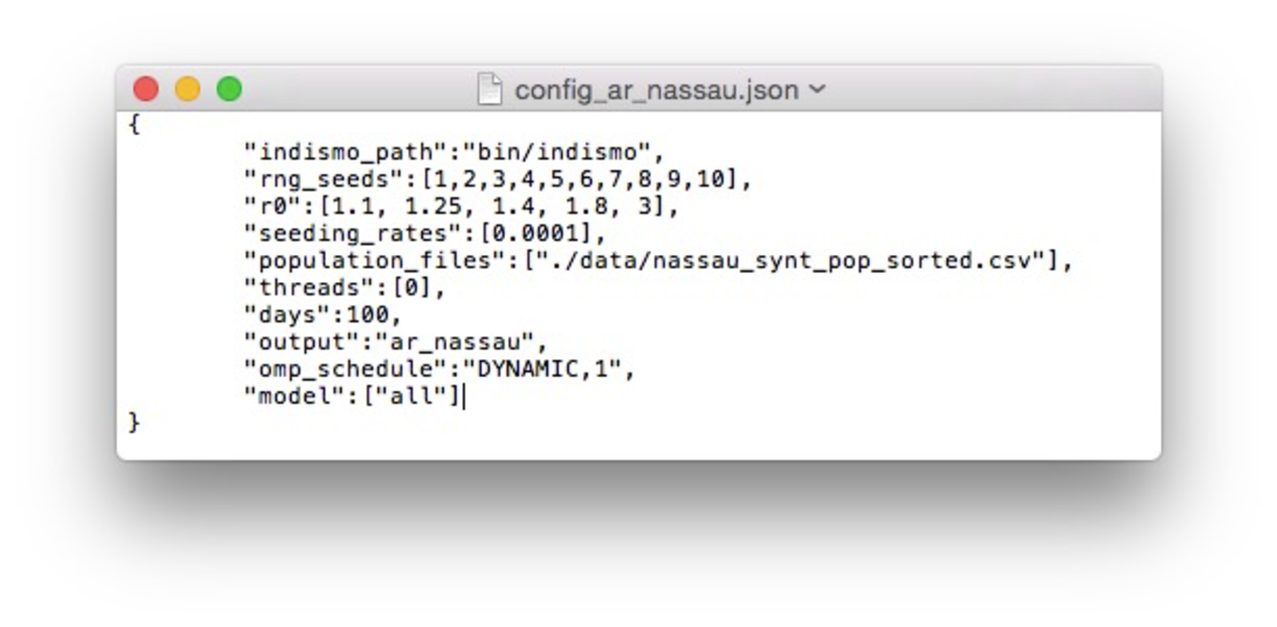
\includegraphics[width=\textwidth]{images/screen_shot_config_file.pdf}  
	\end{center}
	\caption{Screen shot of a $sim\_wrapper$ configuration file.}
	\label{fig:config}
\end{figure}
